\documentclass{article}
\usepackage{geometry}
\geometry{hmargin = 2cm,vmargin = 2cm}
\usepackage[utf8]{inputenc}
\usepackage[T1]{fontenc}
\usepackage[table]{xcolor}
\usepackage{amssymb}
\usepackage{amsmath}
\usepackage{amsthm}
\usepackage{mathrsfs}
\usepackage{graphicx}
\usepackage{listings}
\usepackage{tikz}
\usetikzlibrary{arrows,positioning, calc}
\tikzstyle{vertex}=[draw,fill=white!15,circle,minimum size=20pt,inner sep=0pt]
\usepackage{color}
\definecolor{darkWhite}{rgb}{0.94,0.94,0.94}
\lstset{
  aboveskip=3mm,
  belowskip=-2mm,
  backgroundcolor=\color{darkWhite},
  basicstyle=\footnotesize,
  breakatwhitespace=false,
  breaklines=true,
  captionpos=b,
  commentstyle=\color{red},
  deletekeywords={...},
  escapeinside={\%*}{*)},
  extendedchars=true,
  framexleftmargin=16pt,
  framextopmargin=3pt,
  framexbottommargin=6pt,
  frame=tb,
  keepspaces=true,
  keywordstyle=\color{blue},
  language=python,
  literate=
  {²}{{\textsuperscript{2}}}1
  {⁴}{{\textsuperscript{4}}}1
  {⁶}{{\textsuperscript{6}}}1
  {⁸}{{\textsuperscript{8}}}1
  {€}{{\euro{}}}1
  {é}{{\'e}}1
  {è}{{\`{e}}}1
  {ê}{{\^{e}}}1
  {ë}{{\¨{e}}}1
  {É}{{\'{E}}}1
  {Ê}{{\^{E}}}1
  {û}{{\^{u}}}1
  {ù}{{\`{u}}}1
  {â}{{\^{a}}}1
  {à}{{\`{a}}}1
  {á}{{\'{a}}}1
  {ã}{{\~{a}}}1
  {Á}{{\'{A}}}1
  {Â}{{\^{A}}}1
  {Ã}{{\~{A}}}1
  {ç}{{\c{c}}}1
  {Ç}{{\c{C}}}1
  {õ}{{\~{o}}}1
  {ó}{{\'{o}}}1
  {ô}{{\^{o}}}1
  {Õ}{{\~{O}}}1
  {Ó}{{\'{O}}}1
  {Ô}{{\^{O}}}1
  {î}{{\^{i}}}1
  {Î}{{\^{I}}}1
  {í}{{\'{i}}}1
  {Í}{{\~{Í}}}1,
  morekeywords={*,...},
  numbers=left,
  numbersep=10pt,
  numberstyle=\tiny\color{black},
  rulecolor=\color{black},
  showspaces=false,
  showstringspaces=false,
  showtabs=false,
  stepnumber=1,
  stringstyle=\color{gray},
  tabsize=4,
  title=\lstname,
}
%pour la compilation minted : C:\Users\Serge\Anaconda3\pkgs\pygments-2.2.0-py37_0\Scripts à ajouter en PATH et 
%remplacer pdflatex -synctex=1 -interaction=nonstopmode %.tex
%par pdflatex -synctex=1 -interaction=nonstopmode --shell-escape %.tex
\title{Quadtree}
\author{Tout le monde}
\begin{document}
\maketitle

\newpage

\tableofcontents

\section{Implémentation : comparaison entre structure récursive et représentation en liste}
\subsection{Structure récursive}
Une représentation qui semble la plus naturelle est d'implémenter une structure avec auto-référence. En effet en s'inspirant de la définition inductive on peut voir un arbre binaire comme une structure contenant essentiellement 3 champs : une clef et deux arbres binaires, ses sous-arbres gauche et droit. 
En terme d'implémentation cela dépend du langage utilisé. \\
 En C cela passera par la création d'un type spécifique arbre avec en variable des pointeurs vers des variables de ce même type, en plus d'une variable clef de type entier par exemple. \\
En suivant le paradigme de la programmation objet, on créé une classe arbre ayant deux attributs de type arbre en plus de l'attribut clef (et d'autres attributs si nécessaires). La souplesse de Python sur les types rend la création de la classe particulièrement aisée mais il faudra être vigilant sur l'utilisation. 
On pourra déclarer la classe comme ceci :

\begin{lstlisting}
class ArbreBinaire():
    def __init__(self,clef,gauche = None ,droite = None):
        """ Anything x ArbreBinaire x ArbreBinaire -> ArbreBinaire
        Constructeur d'arbre"""
        self.clef = clef
        self.gauche = gauche
        self.droite = droite
\end{lstlisting}

Exemple d'instanciation :

\begin{lstlisting}
Feuille1 = ArbreBinaire(1)
Feuille2 = ArbreBinaire(2)
Arbre = ArbreBinaire(3,Feuille1,Feuille2)
\end{lstlisting}

L'arbre créé est :
\begin{center}
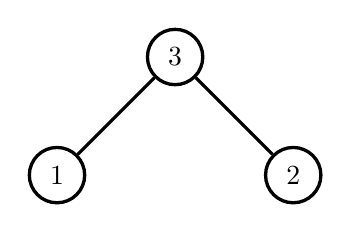
\begin{tikzpicture}[very thick,level/.style={sibling distance=30mm/#1}]
\node [vertex] (r){$3$}
  child {
    node [vertex] (a) {$1$}
   }
   child {
    node [vertex] (a) {$2$}
   }
   
   ;
\end{tikzpicture}
\end{center}

Test Quadtree :
\begin{center}
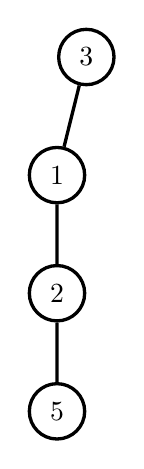
\begin{tikzpicture}[very thick,level/.style={sibling distance=30mm/#1}]
\node [vertex] {$3$}
  child {
    node [vertex, left]  {$1$}
    child {
    	node [vertex] (r) {$2$}
    	child {
    		node [vertex] {$5$}
   		}
   	}
  }

   ;
\end{tikzpicture}
\end{center}
test pour génération python :
\begin{center}
\begin{tikzpicture}[very thick,level/.style={sibling distance=30mm/#1}]


\end{tikzpicture}
\end{center}


\end{document}
